\documentclass{article}
\usepackage[catalan]{babel}
%\usepackage[latin1]{inputenc}   % Permet usar tots els accents i car�ters llatins de forma directa.
\usepackage[utf8]{inputenc}   % Permet usar tots els accents i car�ters llatins de forma directa.
\usepackage{enumerate}
\usepackage{amsfonts, amscd, amsmath, amssymb}
\usepackage[pdftex]{graphicx}
\usepackage{longtable}

\setlength{\textwidth}{16cm}
\setlength{\textheight}{24.5cm}
\setlength{\oddsidemargin}{-0.3cm}
\setlength{\evensidemargin}{0.25cm} \addtolength{\headheight}{\baselineskip}
\addtolength{\topmargin}{-3cm}

\newcommand\Z{\mathbb{Z}}
\newcommand\R{\mathbb{R}}
\newcommand\N{\mathbb{N}}
\newcommand\Q{\mathbb{Q}}
\newcommand\K{\Bbbk}
\newcommand\C{\mathbb{C}}

\newcounter{exctr}
\newenvironment{exemple}
{ \stepcounter{exctr} 
\hspace{0.2cm} 
\textit{Exemple  \arabic{exctr}: }
\it
\begin{quotation}
}{\end{quotation}}


\begin{document}

\textbf{\Large Tema 5. Filtres digitals}

\vskip 0.3 cm
\noindent
\textbf{\large Introducció}

La paraula `filtre' és equivalent a la paraula `sistema', és a dir, fa referència a qualsevol procés que modifica
les característiques d'un senyal d'entrada per donar lloc a un senyal de sortida.
Però en parlar de `filtres' feim èmfasi en que es tracta de sistemes que eliminen o atenuen (filtren) certes característiques 
específiques dels senyals d'entrada mentre conserven o amplifiquen unes altres.

Aquest \textbf{filtratge} pot ésser a nivell \textbf{temporal}, quan s'actua directament sobre els valors temporals del senyal d'entrada,
o bé a nivell \textbf{freqüencial}, quan es modifica directament l'espectre freqüencial del senyal. En tot cas, donat que els nivells
temporal i freqüencial dels senyals estan intimament lligats (mitjançant la transformada de Fourier), tota actuació a nivell temporal
té conseqüències a nivell freqüencial i viceversa.

\vskip 0.3 cm
Exemples: eliminació de renou amb filtre temporal, eliminació d'interferència (xiulet) amb filtratge freqüencial

\vskip 0.3 cm
\textbf{Filtres lineal i no lineals}

 En temes anteriors hem estudiat un tipus particular de sistemes anomenats \textbf{LTI} (lineats i invariants 
amb el temps). El motiu és que es pot fer un estudi sistemàtic del seu comportament. Simplement analitzant la seva resposta davant un impuls unitari (\textbf{resposta impulsional}) es pot calcular la sortida a qualsevol senyal d'entrada (utilitzant l'operació de convolució).
Per aquest motiu, la majoria de filtres que s'utilitzen en la pràctica són de tipus LTI. Un exemple és el filtre de mitjana (veure figura).
No obstant, en segons quins casos és possible utilitzar filtres no lineals. Un exemple de filtre no lineal és el filtre de mediana.

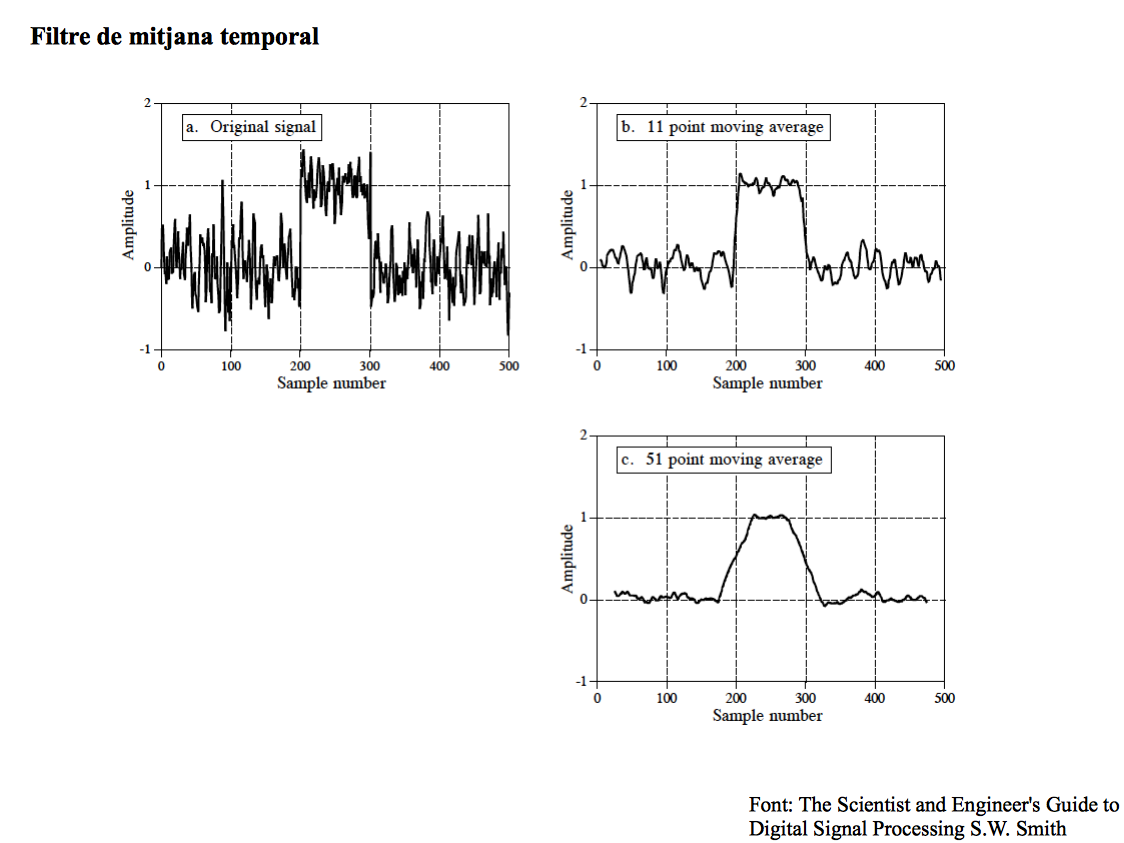
\includegraphics[width=12cm]{mitjanatemp.png}
 
\vskip 0.3 cm
\textbf{Filtres analògics i digitals}

Si aplicam correctament (evitant aliasing) les operacions de conversió A/D i D/A, per qualsevol filtre analògic (circuit electrònic)
podem crear el seu equivalent filtre digital (algoritme executat per un processador). La següent figura mostra un exemple:

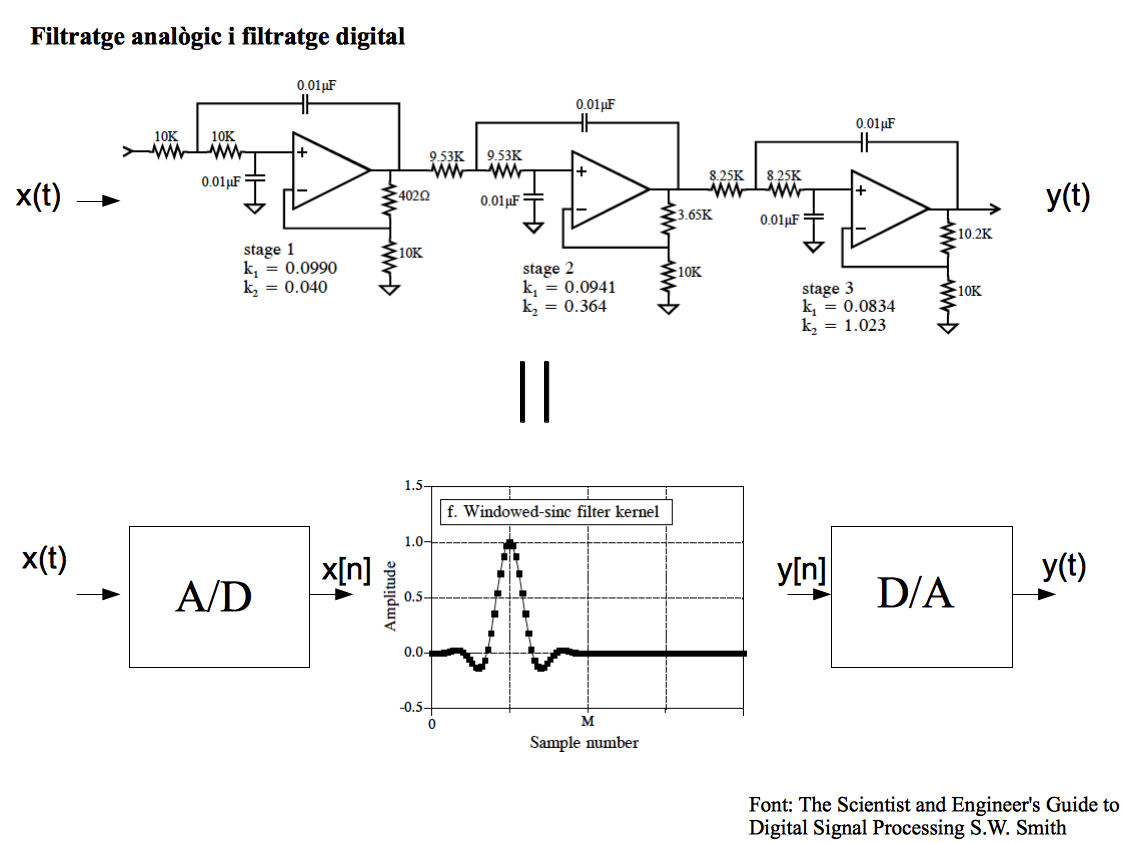
\includegraphics[width=15cm]{analogicvsdigital.png}

\vskip 0.3 cm
\textbf{Filtres FIR i IIR}

Una manera de classificar els filtres LTI és en funció del nombre de mostres que composen la seva resposta impulsional.
Si aquest nombre és finit es diu que són filtres FIR (resposta impusional finita) i en cas contrari es parla de filtres IIR
(resposta impulsional infinita). En principi, pot semblar que només els filtres FIR es poden implementar en la pràctica.
No obstant, hi ha un tipus especial de filtres IIR que es poden escriure de forma iterativa com a funció de l'entrada
i la sortida. Aquests filtres s'anomenen IIR recursius i sí són realitzables, i a més solen ésser més ràpids que els FIR, 
la sortida dels quals es calcula per convolució.


\vskip 0.5 cm
\noindent
\textbf{\large Caracterització temporal dels filtres LTI}

Com ja s'ha comentat en temes anteriors els filtres LTI es caracteritzen per la següent relació entre entrada ($x[n]$) i sortida ($y[n]$):

\[
y[n]=x[n] * h[n]
\]

on `*' representa l'operació de \textbf{convolució}i $h[n]$ és la \textbf{resposta impulsional} del filtre ${\cal T}$ ($h[n]={\cal T}(\delta [n])$).

\vskip 0.3 cm
Una manera alternativa d'estudiar el comportament temporal del filtre és analitzar la seva resposta a l'esglaó unitari ($u[n]$):

\[
h_u[n]={\cal T}(u[n])
\]

Tenim que $h[n]=h_u[n]-h_u[n-1]$, ja que $\delta [n]=u[n]-u[n-1]$.

\vskip 0.3 cm
\textbf{Paràmetres que caracteritzen la resposta freqüencial d'un filtre}

L'estudi de $h_u[n]$ ens permet veure com es comporta el sistema davant canvis bruscs de l'entrada. Els paràmetres a analitzar de $h_u[n]$ 
són (veure figura): 
\begin{itemize}
\item el temps de resposta
\item la saturació (\textit{overshoot})
\item la simetria de la resposta (relacionada amb la linealitat de la fase de la resposta freqüencial, com veurem més endavant)
\end{itemize}

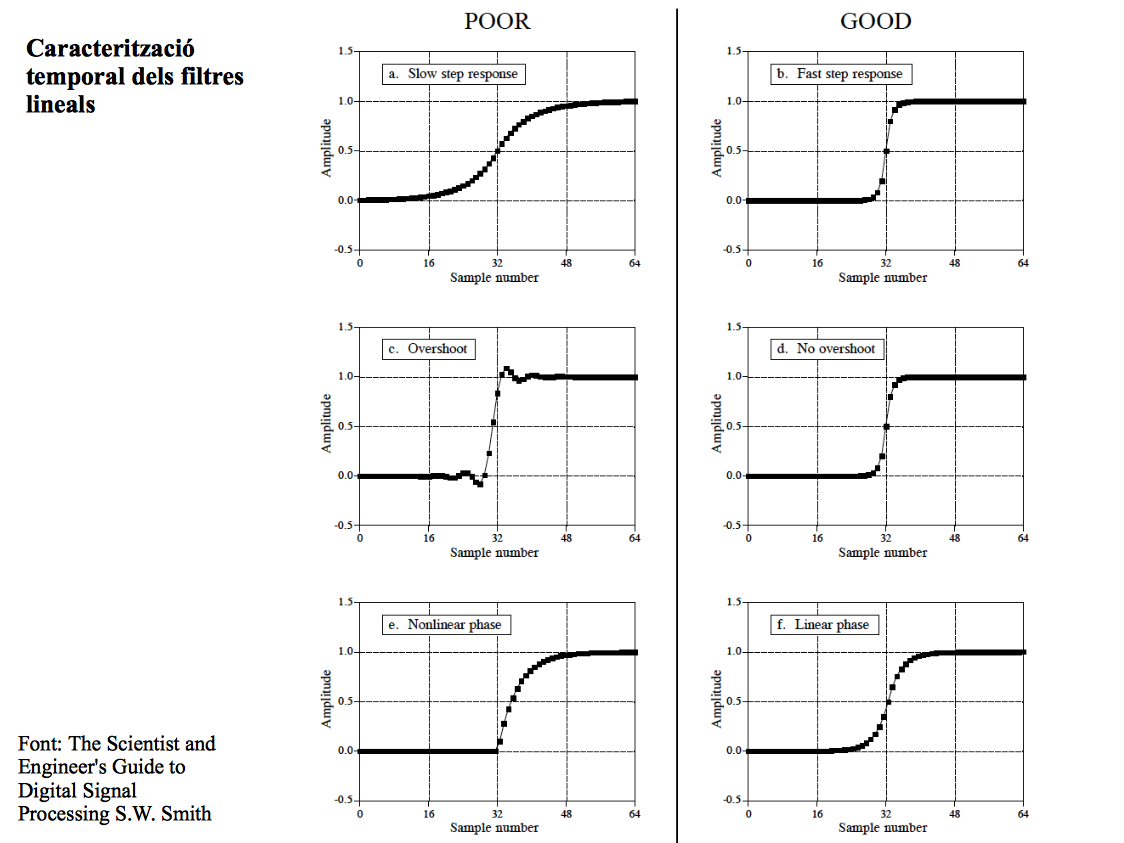
\includegraphics[width=15cm]{cartempfiltres.png}

\vskip 0.3 cm
\textbf{Convolució i FFT}

Una manera pràctica de calcular la convolució d'un senyal d'entrada $x[n]$ amb la resposta impulsional d'un filtre LTI $h[n]$ és amb
l'ajut de la propietat de convolució de la transformada de Fourier:
\[
y[n]= TF^{-1} \{ X(\omega) \cdot H(\omega) \}
\]
on `TF' fa referència a la \textbf{transformada de Fourier en temps discret} i $X(\omega)=TF \{ x[n] \}$ i
$H(\omega)=TF \{ h[n] \}$ (la resposta freqüencial del filtre, de la qual parlarem més endavant).

El problema és que, en la pràctica, no es calcula la transformada de Fourier en temps discret, sino la \textbf{transformada discreta de Fourier},
que és una versió mostrejada de TF: 
\[
DFT\{x[n]\}=X[k] = X(\frac{2\pi}{N}k) \qquad \text{on } \qquad X(\omega)=TF\{x[n]\}
\]

L'ús de la DFT (o la seva implementació algorítmica, la FFT) implica, de manera implícita, considerar que tots els senyals són periódics, de periode
igual al nombre de mostres que els descriu. De manera que, quan calculam $DFT^{-1} \{ X[k]\cdot H[k] \}$ el que feim és equivalent
a convolucionar les versions periòdiques de $x[n]$ i $h[n]$ (a aquesta operació se l'anomena \textbf{convolució circular} de $x[n]$ i $h[n]$), 
per tant no és equivalent (en principi) a la convolució simple dels senyals. Una manera senzilla d'obtenir el resultat desitjat ($x[n] * h[n]$)
utilitzant la DFT és afegint zeros als senyals $x[n]$ i $h[n]$, tal com mostra la següent figura:

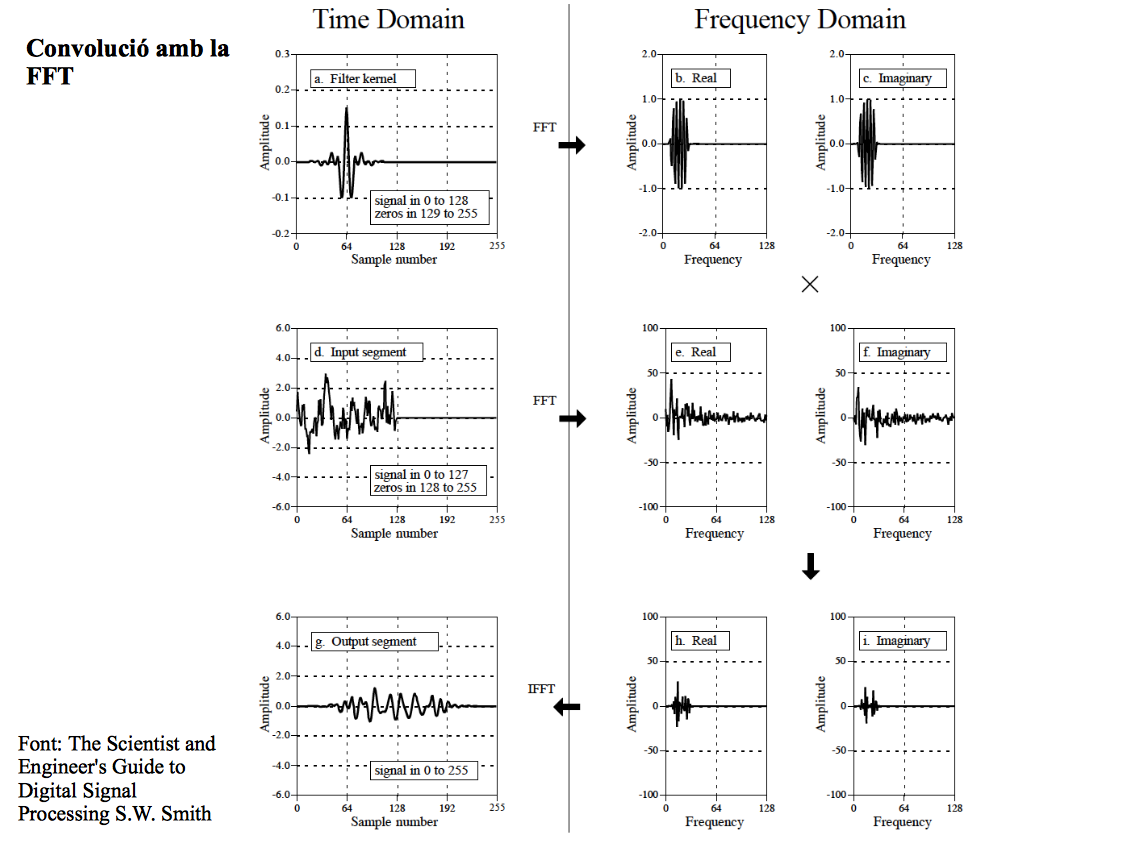
\includegraphics[width=15cm]{fftconv.png}

\vskip 0.5 cm
\noindent
\textbf{\large Caracterització freqüencial dels filtres LTI}

Per a estudiar el comportament freqüencial dels sistemes LTI s'analitza
la sortida d'aquests sistemes quan l'entrada és un to pur (una exponencial 
complexa o una sinusoide).

En general, la sortida d'un sistema LTI amb resposta impulsional $h[n]$ 
quan s'excita amb una entrada $x[n]$ és
\[
y[n]=x[n] * h[n] = \sum_{k=-\infty}^\infty h[k] x[n-k]
\]

En el cas que l'entrada sigui una exponencial complexa $x[n]=A e^{j \omega n}$:
\[
y[n]=\sum_{k=-\infty}^\infty h[k] A e^{j \omega (n-k)}=\left( \sum_{k=-\infty}^\infty h[k] e^{-j \omega k} \right) A e^{j \omega n}=
H(\omega) A e^{j \omega n}
\]

\noindent
on $H(\omega)$ és la transformada de Fourier de $h[n]$. Aquesta transformada existeix si el sistema és estable 
(és a dir, si $\sum_{k=-\infty}^\infty |h[n]| < \infty$).

Si escrivim $H(\omega)$ en funció del seu mòdul i la seva fase ($H(\omega)=|H(\omega)| e^{j \Theta(\omega)}$) llavors
\begin{equation}
y[n]=A |H(\omega)| e^{j (\omega n + \Theta(\omega))}
\end{equation}

Si $h[n]$ pren valors reals $|H(\omega)|$ és una funció parell ($|H(\omega)|=|H(-\omega)|$) i 
$\Theta(\omega)$ és una funció imparell ($\Theta(\omega)=-\Theta(-\omega)$).
En aquest cas la resposta a una sinusoide (sinus o cosinus) és:
\begin{equation}
\begin{array}{l}
y[n]=h[n] * A \cos(\omega n)=A |H(\omega)| \cos(\omega n + \Theta(\omega)) \\ \\
y[n]=h[n] * A \sin(\omega n)=A |H(\omega)| \sin(\omega n + \Theta(\omega)) 
\end{array}
\end{equation}

La conclusió d'aquesta anàlisi és que la resposta d'un sistema LTI davant un senyal sinusoïdal
vé totalment caracteritzada per $|H(\omega)|$ i $\Theta(\omega)$. 
$|H(\omega)|$ determina l'amplificació ($|H(\omega)| > 1$) o atenuació ($|H(\omega)| < 1$)
de l'amplitud de la sinusoide, mentre que $\Theta(\omega)$ determina el desplaçament de fase.
$H(\omega)$ rep el nom de \textbf{resposta freqüencial} del sistema.

\vskip 0.3 cm
\noindent
\textbf{Exemple:} Determinau la resposta del sistema amb resposta impulsional $h[n]=(\frac{1}{2})^n u[n]$
al senyal d'entrada $x[n]=10 - 5 \sin \frac{\pi}{2} n + 20 \cos \pi n$


\vskip 0.3 cm
\textbf{Classificació dels filtres en funció de la seva resposta freqüencial}

Es parla de filtres freqüencials quan ens referim als sistemes
que permeten passar (amb poca o cap atenuació) senyals d'unes determinades freqüències
(\textbf{banda de pas})
i que atenuen (total o parcialment) senyals d'altres freqüencies (\textbf{banda de stop}).

Els \textbf{filtres ideals} són aquells que atenuen totalment una banda de freqüències
i deixen passar sense modificació una altra banda de freqüències. La magnitud 
de la seva resposta freqüencial es de la forma:
\[
|H(\omega)|=\begin{cases} 1 & \text{si } \omega_1 < \omega < \omega_2 \\ \\
0 & \text{altrament} \end{cases}
\]

En funció dels valors de $\omega_1$ i $\omega_2$ es parla de filtres passa-baix,
passa-banda, passa-alt, de banda eliminada o passa-tot:

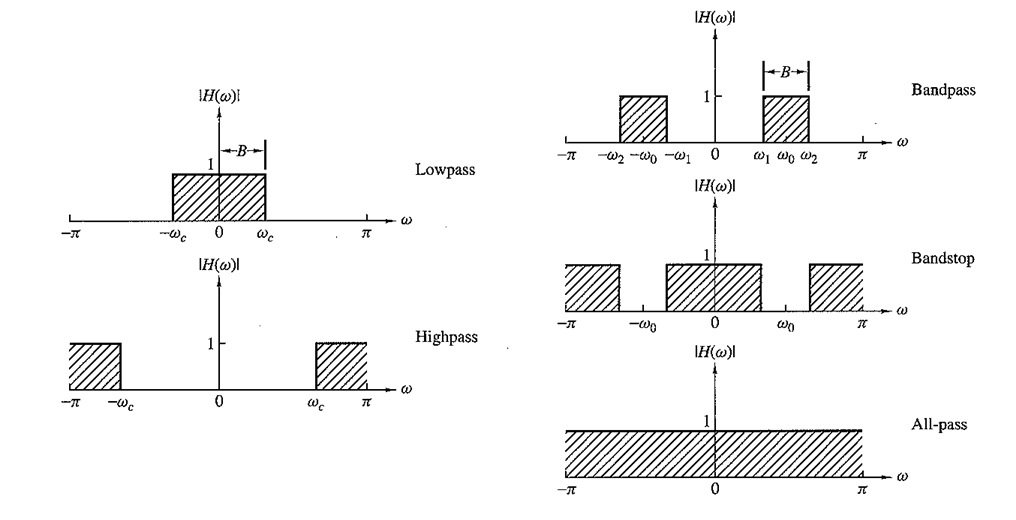
\includegraphics[width=15cm]{idealfilters.png}


\vskip 0.3 cm
\textbf{Paràmetres que caracteritzen la resposta freqüencial d'un filtre}

L'estudi de $H(\omega)$ ens permet veure com es comporta el filtre davant les diferents freqüències que composen el senyal d'entrada. 
Els paràmetres a analitzar de $H(\omega)]$ són (veure figura): 
\begin{itemize}
\item el decreixement (\textit{roll-off})
\item les oscilacions de la banda de pas
\item l'atenuació a la banda de stop (en escala logarítmica - dB -)
\end{itemize}

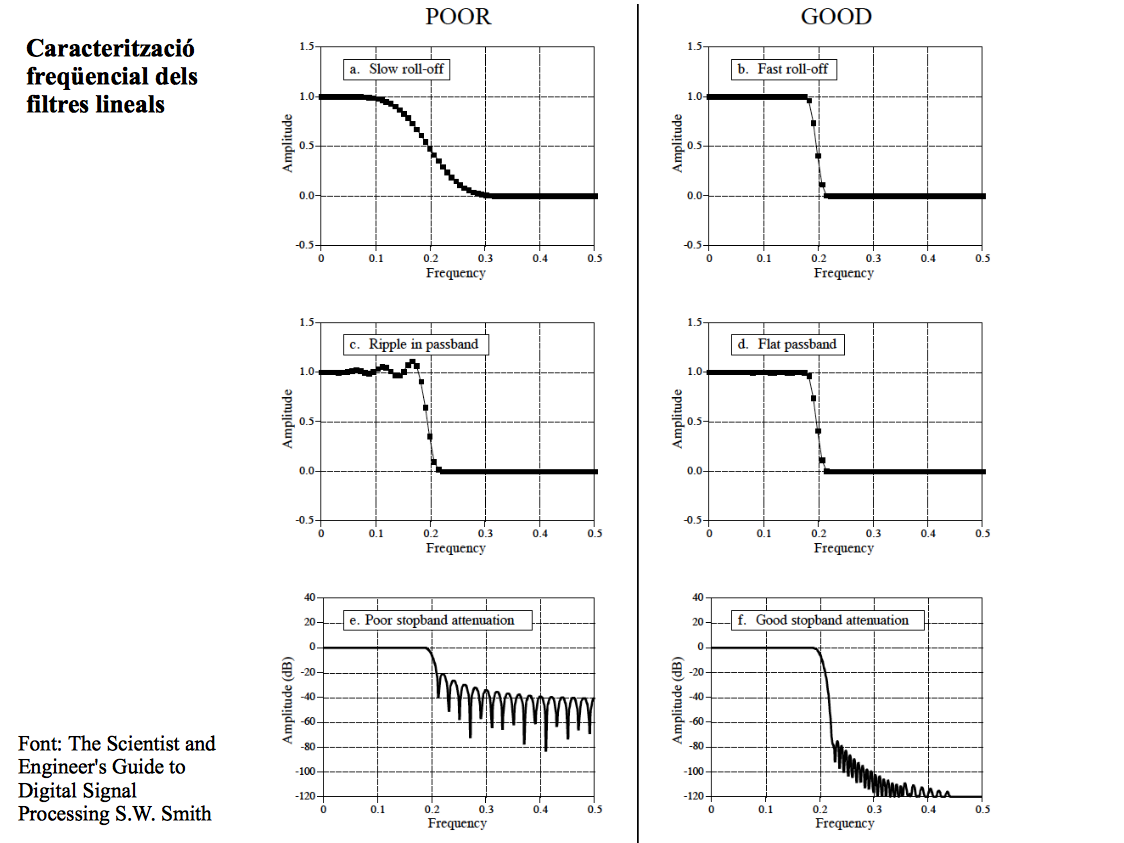
\includegraphics[width=15cm]{carfreqfiltres.png}

\vskip 0.3 cm
\textbf{Anàlisi freqüencial de filtres descrits per una funció de transferència racional. Posició de pols i zeros i comportament del filtre}

Consideram ara el cas dels sistemes LTI que es poden descriure amb una funció de transferència
(transformada Z de la resposta impulsional) racional.

\[
H(z)=\frac{\sum_{k=0}^M b_k z^{-k}}{1+ \sum_{k=0}^N a_k z^{-k}}=
b_0 \frac{ \Pi_{k=1}^M (1-z_k z^{-1}) }{ \Pi_{k=1}^N (1-p_k z^{-1}) }
\]

Recordem que si la ROC de $H(z)$ conté el cercle unitat llavors $H(\omega)=H(z)|_{z=e^{j\omega}}$, per tant
\[
H(\omega)=b_0 \frac{ \Pi_{k=1}^M (1-z_k e^{-j\omega}) }{ \Pi_{k=1}^N (1-p_k e^{-j\omega}) }
\]

També podem trobar l'expressió de $|H(\omega)|^2$ en funció de la transformada Z per a sistemes amb $h[n]$ real:
\[
|H(\omega)|^2=H(\omega) H^*(\omega)=H(\omega) H(-\omega)=H(z) H(z^{-1})|_{z=e^{j\omega}}
\]


Per últim, a partir de l'expressió 
\[
H(\omega)=b_0 \frac{ \Pi_{k=1}^M (1-z_k e^{-j\omega}) }{ \Pi_{k=1}^N (1-p_k e^{-j\omega}) }=
b_0 e^{j \omega (N-M)} \frac{ \Pi_{k=1}^M (e^{j\omega}-z_k) }{ \Pi_{k=1}^N (e^{j\omega}-p_k) }
\]

podem interpretar la relació entre la posició dels pols i zeros de $H(z)$ i la resposta freqüencial
del sistema. Si $e^{j\omega} \simeq z_k$ per a algun $z_k$, llavors $H(\omega) \simeq 0$, per tant 
els zeros pròxims al cercle unitat fan que la resposta a sinuosides amb freqüència propera al zero
sigui petita. En canvi, si $e^{j\omega} \simeq p_k$ per a algun $p_k$, llavors $H(\omega) \simeq \infty$, per tant 
els pols pròxims al cercle unitat fan que la resposta a sinuosides amb freqüència propera al pol
sigui gran (veure figura).

\begin{center}
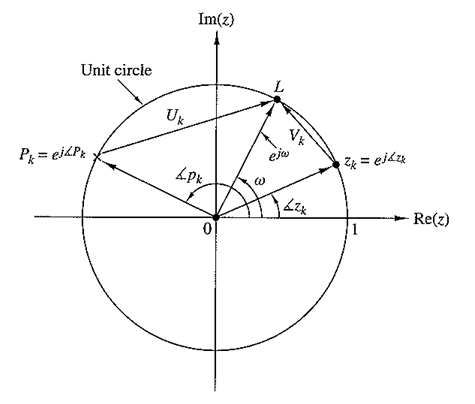
\includegraphics[width=8cm]{polszerosHomega.png}
\end{center}

\vskip 0.3 cm
\textbf{Exemple:} Raonau perquè el sistema descrit per la funció de transferència $H(z)=\frac{1}{1-0.8z^{-1}}$
té un pic de la magnitud de la resposta freqüencial a $\omega=0$.
 

\vskip 0.3 cm
A partir de l'analisi de la relació entre la posició dels pols i zeros del sistema i la seva
resposta freqüencial (veure secció anterior) podem deduir si un sistema és passa-baix, passa-alt
o passa-banda observant el seu diagrama de pols i zeros. La figura següent
mostra un exemple per als casos dels filtres passa-baix i passa-alt. 
Aquesta propietat s'utilitza per dissenyar filtres
amb un determinat comportament freqüencial. 

\begin{center}
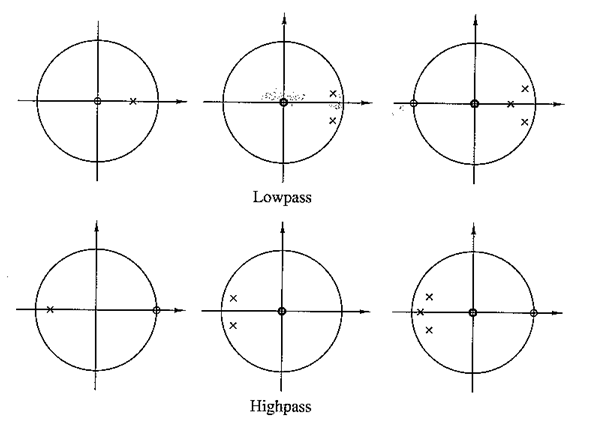
\includegraphics[width=10cm]{polszerosfiltres.png}
\end{center}


\vskip 0.3 cm
Per al cas dels filtres passa tot tenim que 
\[
|H(\omega)|=1 \quad \forall \omega \qquad \text{equivalent a } \quad |H(\omega)|^2=1 \quad \forall \omega
\]

Si la funció de transferència del sistema s'escriu com una funció racional l'anterior relació
implica que $H(z)$ és de la forma 
\[
H(z)=z^{-N} \frac{A(z^{-1})}{A(z)}
\]

\noindent
ja que llavors
\[
|H(\omega)|^2=H(z) H(z^{-1})|_{z=e^{j\omega}}= z^{-N} \frac{A(z^{-1})}{A(z)} z^{N} \frac{A(z)}{A(z^{-1})}|_{z=e^{j\omega}}= 1
\]

En aquest cas, si $z_0$ \'es un pol de $H(z)$, llavors $\frac{1}{z_0}$ ha d'ésser un zero de $H(z)$ i viceversa.
La figura següent mostra dos exemples de diagrames de pols i zeros per a filtres passa-tot.

\begin{center}
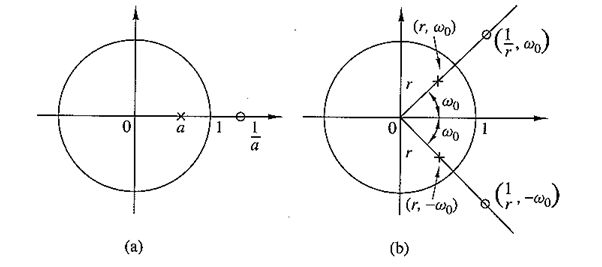
\includegraphics[width=10cm]{polszerospassatot.png}
\end{center}






\vskip 0.3 cm
Un filtre és diu de \textbf{fase mínima} si tots els pols i els zeros de la seva funció de transferència
es troben a l'interior del cercle unitat. 

Si la funció de transferència és de la forma $H(z)=\frac{B(z)}{A(z)}$ i el filtre és
de fase mínima llavors:
\begin{itemize}
\item el filtre és estable i causal
\item el filtre és \textbf{invertible}, és a dir, existeix una funció $H_I(z)$ tal que $H(z) H_I(z)=1$.
En aquest cas $H_I(z)=\frac{1}{H(z)}=\frac{A(z)}{B(z)}$
\item el filtre invers és estable i causal
\end{itemize}

Una darrera propietat relativa als filtres de fase mínima és que la funció de transferència de
qualsevol filtre amb fase no mínima és pot escriure com el producte de les funcions de
transferència d'un filtre de fase mínima i un filtre passa tot:

\[
H(z)=H_{\text{min}}(z) H_{\text{pt}}(z)
\]

En particular, si el filtre és estable i causal amb $H(z)=\frac{B(z)}{A(z)}$ i 
$B(z)$ es pot descomposar com $B(z)=B_1(z) B_2(z)$,
on $B_1(z)$ té totes les seves arrels dins el cercle unitat i $B_2(z)$ fora del cercle unitat,
llavors 
\[
H_{\text{min}}(z)=\frac{ B_1(z) B_2(z^{-1}) }{A(z)}
\qquad 
H_{\text{pt}}(z)=\frac{B_2(z)}{B_2(z^{-1})}
\]
\noindent
on $B_2(z^{-1})$ és un polinomi amb totes les seves arrels dins el cercle unitat i $A(z)$ té també 
totes les seves arrels dins el cercle unitat ja que el filtre és estable i causal. 


\vskip 0.3 cm
\textbf{Filtres de fase lineal}

En les seccions anteriors s'han definit els filtres ideals com aquells que tenen una magnitud 
de la resposta freqüencial igual a $1$ en una determinada banda de freqüències i $0$ fora
d'ella, però no hem parlat de la fase de la resposta freqüencial.

Direm que un filtre és de \textbf{fase lineal generalitzada} si $\Theta(\omega)=-\omega \alpha + \beta$.
Si $\beta=0$ direm que el filtre és de fase lineal. Anem a estudiar el comportament
dels filtres amb fase lineal generalitzada.

Sigui un filtre digital amb $h[n]$ real i resposta freqüencial
\[
H(\omega)=\begin{cases} C e^{-j( \omega \alpha - \beta)} & \text{si } \omega_1 < \omega < \omega_2 \\ \\
0 & \text{altrament} \end{cases}
\]

La resposta d'aquest filtre a un senyal sinusoïdal amb freqüencia $\omega \in (\omega_1, \omega_2)$ és:
\begin{equation}
\begin{array}{l}
y[n]=h[n] * \cos(\omega n)=A C \cos(\omega (n - \alpha) + \beta) \\ \\
y[n]=h[n] * \sin(\omega n)=A C \sin(\omega (n - \alpha)+ \beta)
\end{array} 
\end{equation}

És a dir, la sortida del sistema és una versió atenuada, retardada i desplaçada en fase del senyal d'entrada.
Malgrat que aquest comportament del filtre estigui lluny del comportament ideal (voldriem un senyal idèntic
al d'entrada a la sortida), el fet que per a totes les freqüències $\omega \in (\omega_1, \omega_2)$ es tengui
la mateixa atenuació, retard i desplaçament de fase fa que, per a senyals compostos per vàries freqüències,
el senyal de sortida tengui la mateixa \textit{forma} que el d'entrada (no hi ha \textit{distorsió}). 
Això no passaria si cada freqüència
es veiés afectada de forma diferent pel filtre. És per aquest motiu que els filtres amb fase lineal generalitzada
es consideren \textit{suficientment bons} per al filtratge de senyal i no s'exigeix que els filtres ideals
tenguin fase $0$ ($\Theta(\omega)=0$).


\vskip 0.3 cm
\textbf{Filtres FIR de fase lineal generalitzada}

Considerem el cas general d'un filtre FIR causal de longitud $M+1$:
\[
h[n]=\{ h[0], h[1], \cdots, h[M-1], h[M] \}
\]

Es pot demostrar que el filtre és de fase lineal generalitzada si 
\[
h[n]=\pm h[M-n] \qquad \forall n=0, 1, \cdots, M
\]

(la implicació inversa no és certa, és a dir, un filtre pot ésser de fase lineal
sense verificar l'anterior relació).

Aquesta condició implica que la transformada Z de $h[n]$ ha de verificar:
\[
z^{-M}H(z^{-1})=\pm H(z)
\]
\noindent
És a dir, les arrels del polinomi $H(z)$ també són arrels de $H(z^{-1})$, la qual cosa significa que si
$z_i$ és zero de $H(z)$ llavors $\frac{1}{z_i}$ també ho és. A més, si $h[n]$ és real llavors
les arrels complexes han de formar parells conjugats i per tant, si $z_i$ és zero de $H(z)$ llavors
$z_i^*$,$1/z_i$ i $1/z_i^*$ també són arrels. La Figura \ref{zerosFIRlineal} mostra un exemple
de la distribució dels zeros en un filtre FIR causal real de fase lineal.

\begin{figure}[htbp]
\begin{center}
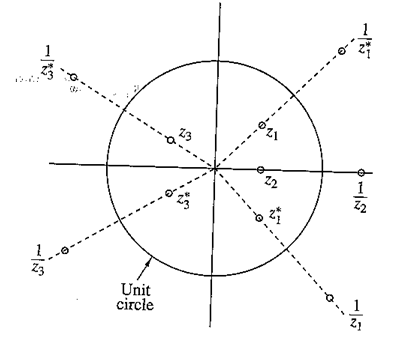
\includegraphics[width=5cm]{zerosFIRlineal.png}
\end{center}
\caption{Exemple de la distribució dels zeros en un filtre FIR causal real de fase lineal.}
\label{zerosFIRlineal}
\end{figure}

\vskip 0.2 cm
Si $h[n]=h[M-n]$ és diu que el filtre FIR de fase lineal és \textbf{simètric}.
Si $h[n]=-h[M-n]$ és diu que el filtre és \textbf{antisimètric}. En ambdos casos es pot distingir
entre els filtres amb un nombre de mostres ($M+1$) parell o imparell. Això dóna lloc
a quatre configuracions possibles per als filtres FIR de fase-lineal:
tipus I (simètric imparell), tipus II (simètric parell), tipus III (antisimètric imparell)
i tipus IV (antisimètric parell). Les figures següents mostren un exemple de cada tipus
i la magnitud de les seves respostes en freqüència. (Font: Discret-Time Signal
Processing, A. Oppenheim, W. Schafer, Prentice-Hall, 1989).
Observam que els filtres tipus I i II són filtres passa-baix, els tipus III passa banda 
i el tipus IV passa-alt.


\begin{center}
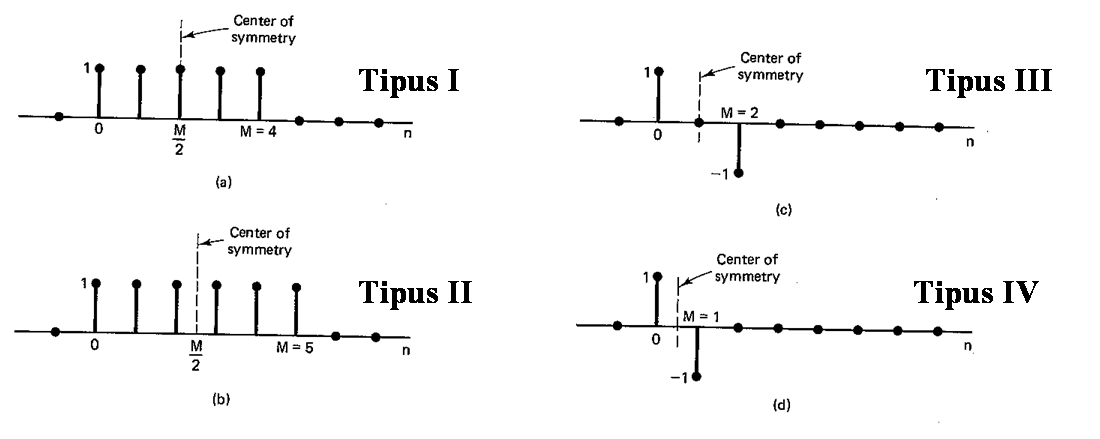
\includegraphics[width=12cm]{tipusFIR.png}
\end{center}

\begin{center}
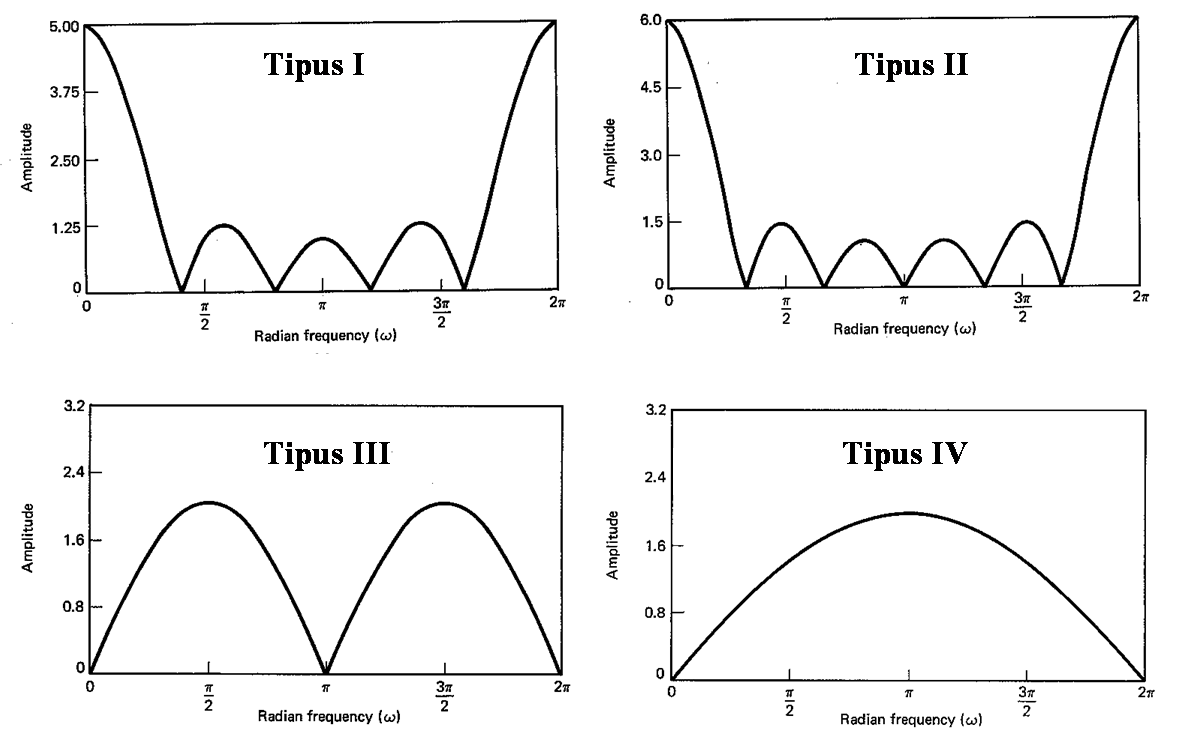
\includegraphics[width=12cm]{tipusFIR_H.png}
\end{center}


\vskip 0.5 cm
\noindent
\textbf{\large Disseny de filtres freqüencials}

\vskip 0.2 cm
\textbf{El problema de la no-causalitat dels filtres ideals}

Considerem un filtre passa-baix ideal amb funció de transferència
\[
H(\omega)=\begin{cases} 1 & \text{si } |\omega| \leq \omega_c \\ 0 & \text{altrament} \end{cases}
\]

La transformada inversa d'aquesta funció dóna com a resposta impulsional
\[
h[n]=\begin{cases} \frac{\omega_c}{n} & \text{si } n=0 \\ 
\frac{\omega_c}{n} \mathrm{sinc}(\omega_c n) & \text{altrament} \end{cases}
\]

Observam (figura inferior)  que aquesta resposta impulsional correspon a un filtre no causal i per tant és \textbf{irrealitzable}.
En general obtenim el mateix resultat per a qualsevol filtre ideal: qualsevol filtre per al qual
$|H(\omega)|=0$ en un interval de freqüències (cas de tots els filtres ideals) és un filtre no causal i per
tant irrealitzable.


\begin{center}
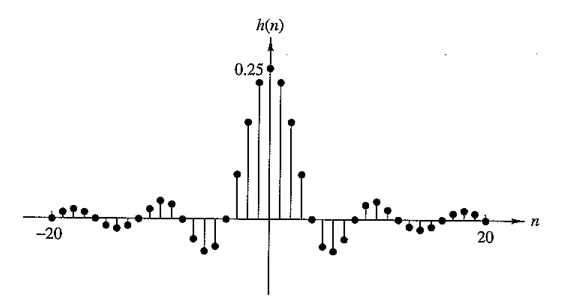
\includegraphics[width=8cm]{passabaixideal.png}
\end{center}

\vskip 0.3 cm
Una manera d'incrementar la `realitzabilitat' del filtre consisteix en desplaçar a la dreta la seva resposta impulsional, de manera que la majoria de
valors amb una magnitud important corresponguin a instants de temps positius. A nivell freqüencial això implica multiplicar la resposta 
en freqüència original per una exponencial complexa, és a dir, obtenir un filtre de fase lineal:

\[
H_k(\omega)=TF\{ h[n-k] \}=e^{-j\omega k} H(\omega) \qquad \rightarrow \qquad \text{Fase}(H_k(\omega))=-j\omega k
\]

\vskip 0.3 cm
Encara així, per a que el filtre `desplaçat' sigui realitzable s'han de truncar (posar a zero) els valors amb índexos negatius i, per simetria,
també els positius a partir d'un cert valor de `n' (la conservació de la simetria permet tenir encara un filtre de fase lineal). 
El fet de truncar la resposta impulsional del filtre implica obtenir un comportament oscil.latori de la seva resposta impulsional, degut
a l'efecte de Gibbs (veure figura).


\begin{center}
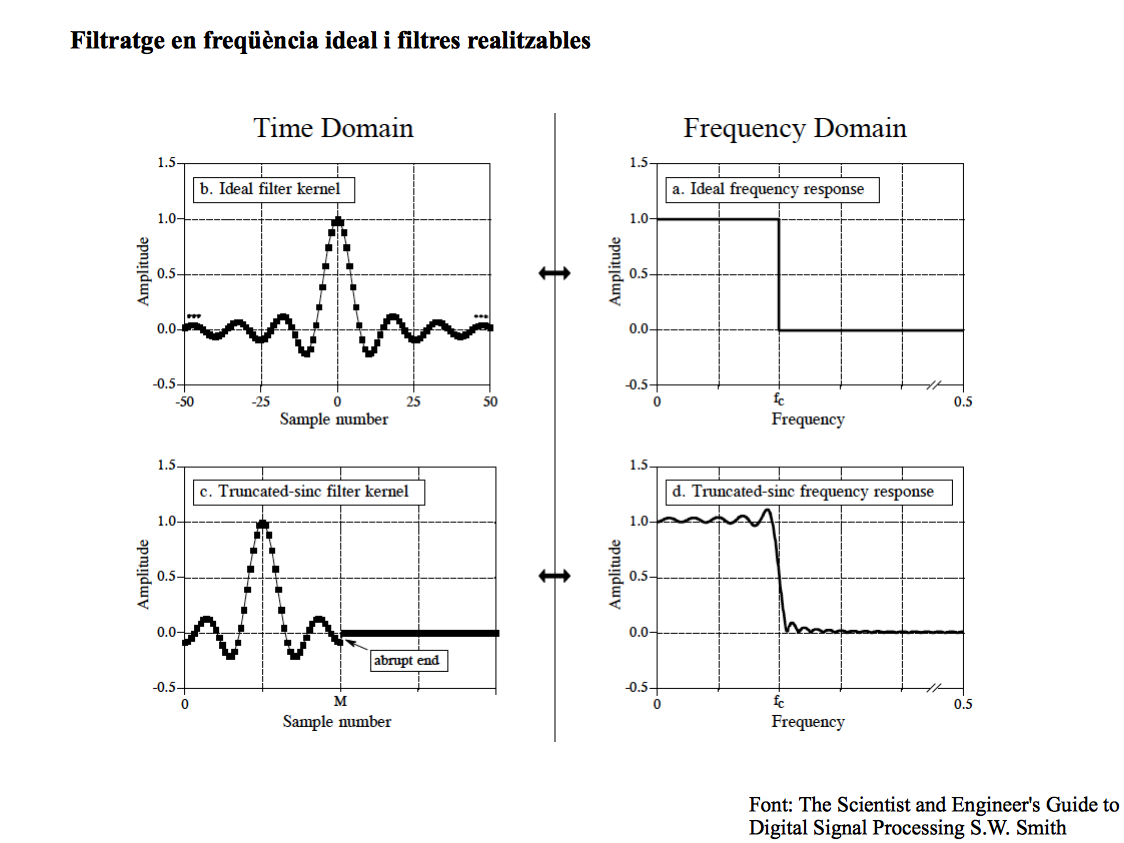
\includegraphics[width=12cm]{filtreidealrealitzable.png}
\end{center}


\vskip 0.3 cm
\textbf{Disseny de filtres FIR de fase lineal mitjançant finestres}

Una manera de suavitzar les oscil.lacions del filtre obtingut per desplaçament + truncament del filtre ideal 
consisteix en multiplicar la resposta impulsional del filtre per una funció que pren valors decreixents a mida que l'índex 
s'allunya de la posició màxima del filtre (veure figura). 
Aquesta funció rep el nom de `finestra' i n'hi ha de diferents tipus (Blackman, Hamming, etc).
El filtre resultant s'anomena \textbf{windowed sinc}.

\begin{center}
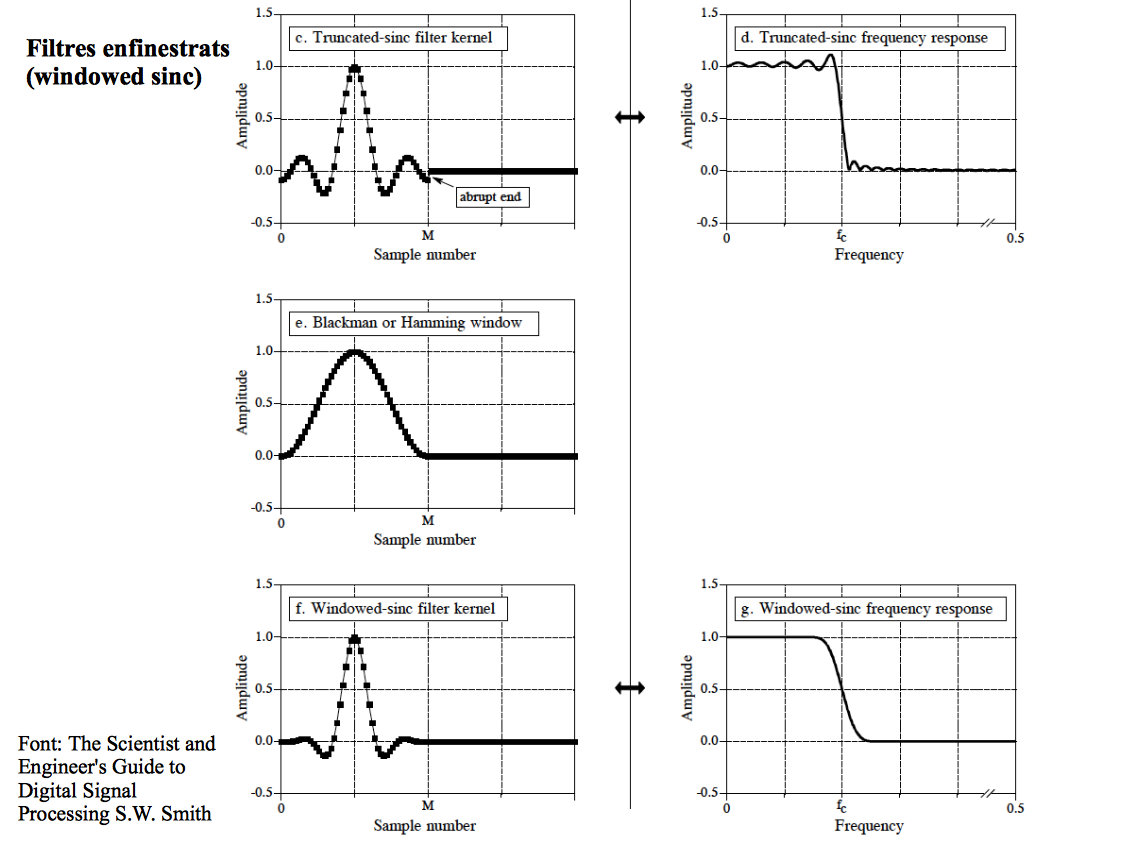
\includegraphics[width=13cm]{windowedsinc.png}
\end{center}


\vskip 0.3 cm
\textbf{Disseny de filtres FIR de fase lineal per mostreig de freqüències}

En aquest cas s'especifica la resposta freqüencial desitjada ($H_d(\omega)$) per a un conjunt discret de freqüències $\omega_k$
i es troben els valors de $h[n]$ resolent un sistema d'equacions.

\vskip 0.3 cm
\textbf{Disseny de filtres FIR de fase lineal òptims}

Els mètodes de disseny anterior no permeten controlar de manera precisa les freqüències de
separació de la banda de pas i la de stop.
Els filtres FIR de fase lineal òptims minimitzen la diferència entre les respostes del filtre
ideal i el filtre dissenyat en cada una de les bandes. L'equació d'aquest filtres es troba
resolent un problema de minimització, seguint una tècnica formulada per Txebytxev.

\vskip 0.3 cm
\textbf{Disseny de filtres IIR}

Les tècniques de disseny de filtres IIR es basen en la conversió de filtres analògics a filtres
digitals. Els filtres analògics es dissenyen per a verificar una sèrie d'especificacions,
seguint unes tècniques de disseny ben conegudes en l'àrea del processament analògic: disseny
tipus Butterworth o disseny tipus Txebyshev. La figura següent mostra un exemple
de la forma de la resposta freqüencial de cada tipus de filtre (Butterworth, esquerra. Txebytxev, dreta). 
La conversió de les expresions
obtingudes al cas discret es fa mitjançant un canvi de variables (transformació bilineal).

\begin{center}
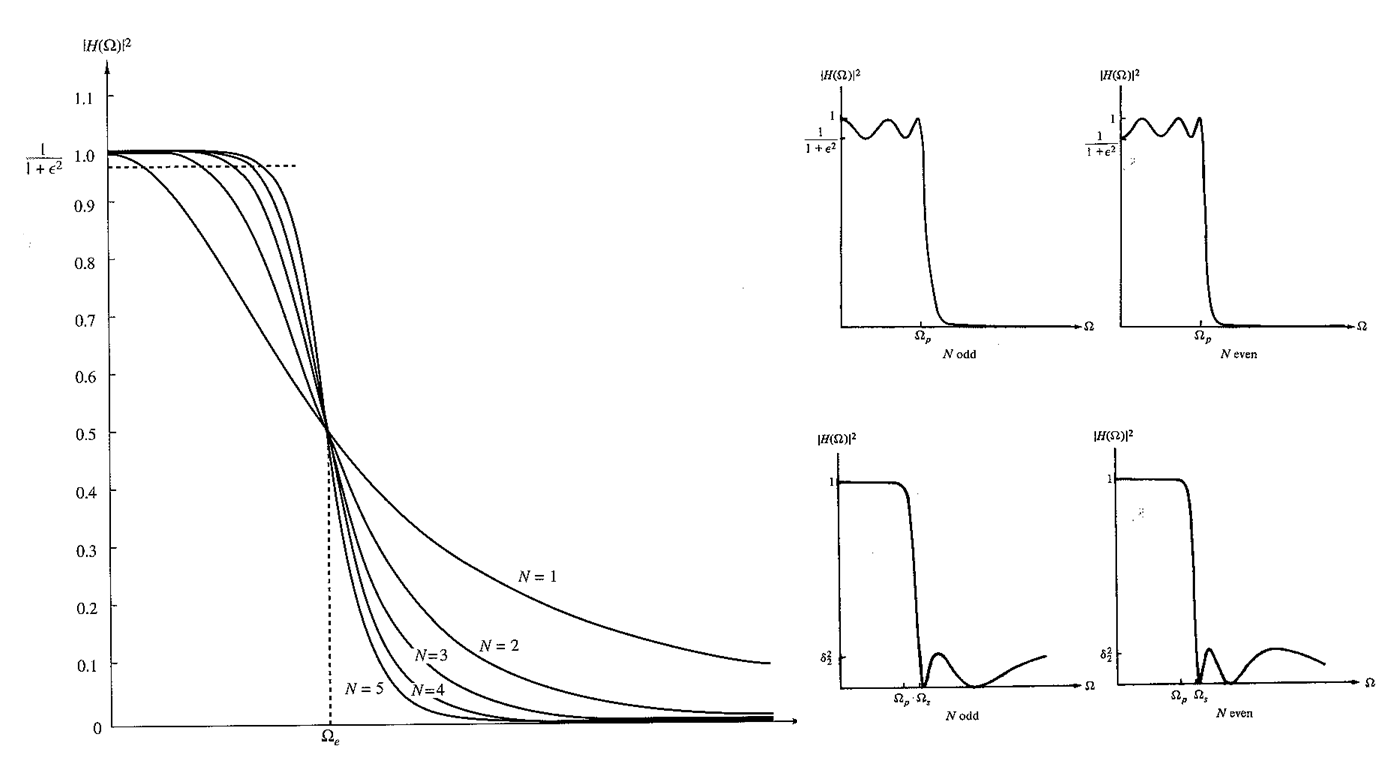
\includegraphics[width=12cm]{ButtTxeby.png}
\end{center}


\vskip 0.5 cm
\noindent
\textbf{\large Comporació del comportament freqüencial i temporal dels filtres analògics i digitals}

En general podem dir que els filtres digitals superen als analògics en termes del seu comporatment 
tant freqüencial com temporal (veure figura) i també per la seva flexibilitat. No obstant, en aplicacions on el rang 
de resposta (tant temporal com freqüencial) ha d'ésser molt gran, és necessari utilitzar filtres analògics,
ja que no necessiten emmagatzemar ingents quantitats de dades per fer el processament. 
A més, com no necessitem les etapes de conversió A/D i D/A, són més ràpids que els digitals.
 
\begin{center}
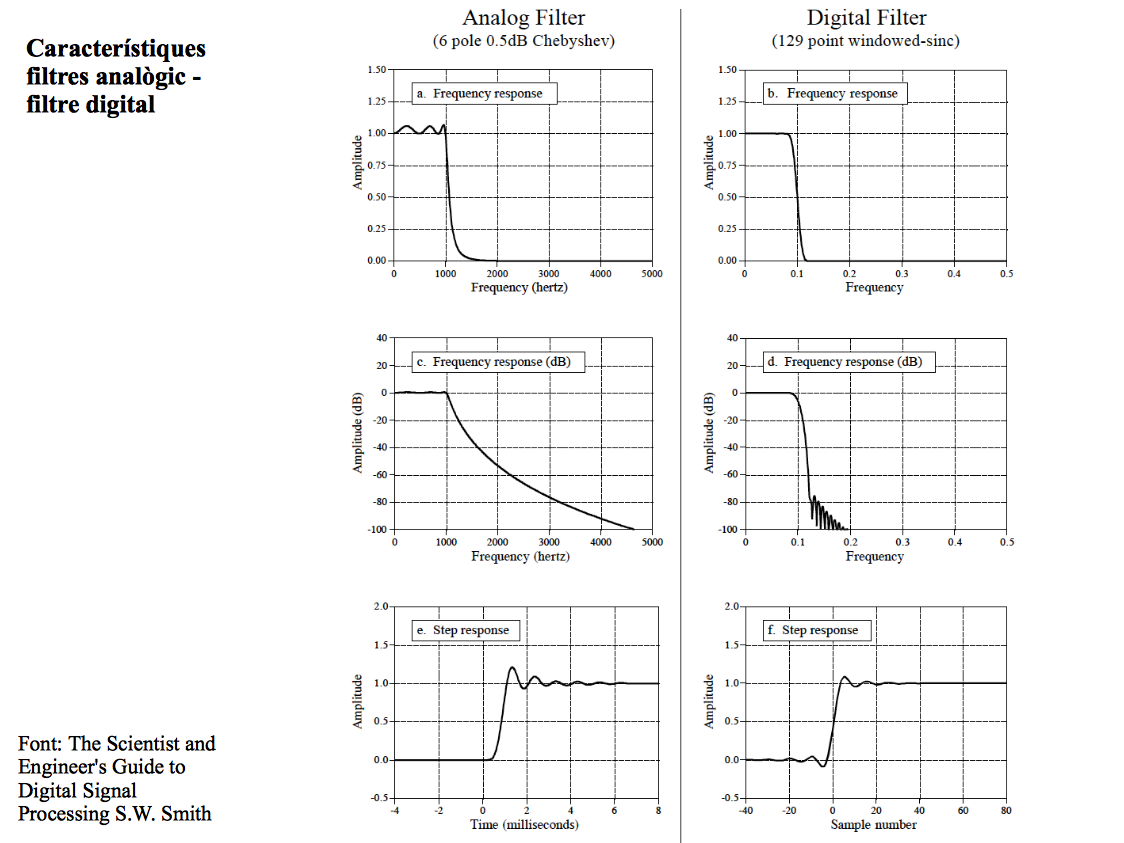
\includegraphics[width=15cm]{caranalogicdigital.png}
\end{center}



\vskip 7cm
\noindent
\textbf{Nota:} algunes de les figures d'aquest cap\'itol s'han tret de Digital Signal Processing, J. Proakis, D. Manolakis, Pearson Prentice Hall, 2007.


\end{document}



